\documentclass[aps,prApplied,twocolumn,superscriptaddress,floatfix]{revtex4-2}

\usepackage{amsmath,amssymb}
\usepackage{graphicx}
\usepackage{hyperref}
\usepackage{xcolor}
\usepackage{listings}
\usepackage{booktabs}
\usepackage{siunitx}
\sisetup{detect-all=true, per-mode=symbol}

\lstset{
  basicstyle=\ttfamily\small,
  breaklines=true,
  frame=single,
  columns=fullflexible,
  keepspaces=true,
  showstringspaces=false,
}

\hypersetup{
  colorlinks=true,
  linkcolor=blue!60!black,
  citecolor=blue!60!black,
  urlcolor=blue!60!black,
}

\begin{document}

\title{OpenQHAL: A Portable Quantum Pulse Compiler with\\
Compiler--Decoder Co-Design for qLDPC Codes}

\author{11-qlab}
\affiliation{Open-source quantum infrastructure, \url{https://github.com/11-qlab}}

\date{\today}

\begin{abstract}
We present \textsc{OpenQHAL}, a portable quantum pulse compiler and
hardware abstraction layer (HAL) that compiles logical circuits to
per-channel I/Q waveforms, schedules syndrome extraction for quantum
low-density parity-check (qLDPC) codes, and bridges the
compiler--decoder interface through a check-annotated detector error
model. \textsc{OpenQHAL} exposes a frozen C ABI with four backend
implementations---a statevector simulator, an IBM Quantum backend via
Qiskit Runtime, a QICK/RFSoC driver, and a Zurich HDAWG driver---plus a
Python abstract base class that allows new backends to be added without
recompilation. We validate the compiler end-to-end on IBM's
156-qubit Heron~r2 processor, obtaining Bell-state fidelity
\num{98.2}\%, GHZ-3 fidelity \num{97.1}\%, and GHZ-4 fidelity
\num{95.6}\%, consistent with published device characteristics. We
construct the $[[144,12,12]]$ Bivariate Bicycle code, schedule its
syndrome extraction at depth~7---matching the published lower bound
that depth~6 is unattainable---and demonstrate BP+OSD decoding with a
threshold near physical error rate $p \approx \num{0.006}$. Latency
measurements on cloud hardware show that \num{99.99}\% of wall-clock
time is network and queue, not compilation; the HAL's contribution is
invisible at cloud timescales, which is precisely why a portable
abstraction is essentially free.
\end{abstract}

\maketitle

\section{Introduction}
\label{sec:intro}

Quantum computing faces a software infrastructure problem. Every
laboratory builds its own pulse-level control stack, badly. Calibration
lives in notebooks, pulse sequences are hardcoded for specific hardware,
channel mappings are ad-hoc, and reproducing results across devices is a
manual, error-prone process. When Qiskit Pulse was deprecated in
2024~\cite{qiskit-pulse-deprecation}, no portable replacement existed.

Meanwhile the field has converged on a target: fault-tolerant quantum
computation via quantum low-density parity-check (qLDPC)
codes~\cite{bravyi2024high}. The $[[144,12,12]]$ Bivariate Bicycle (BB)
code encodes 12 logical qubits with distance 12---a $12\times$ overhead
reduction over surface codes at matched distance. But qLDPC codes expose
a compiler--decoder co-design (CDCD) problem that no existing framework
addresses: the decoder requires a circuit-level noise model that depends
on the compiler's physical layout, while the compiler requires the
decoder's error model to schedule syndrome extraction optimally. This
circular dependency is named as unsolved in the 2026
survey~\cite{zhu2026ftqc}.

This paper makes three contributions:
\begin{enumerate}
  \item A portable HAL with a frozen C ABI, four backends, and no
        changes required above the ABI when switching hardware.
  \item A CDCD bridge that annotates compiled pulse programs with qLDPC
        check structure and produces per-check detector error models for
        the decoder.
  \item Hardware validation on IBM's Heron~r2 processor, including a
        qLDPC syndrome extraction circuit compiled through the full
        pipeline.
\end{enumerate}

We also report a hardware constraint discovered during validation:
IBM's backend compiler rejects mid-circuit reset instructions that have
not been converted by an explicit \texttt{ConvertToMidCircuitReset\-AndMeasure}
transpiler pass (error 6056).

\section{Architecture}
\label{sec:arch}

\subsection{Layer separation}

\textsc{OpenQHAL} separates three concerns usually tangled together:
\begin{itemize}
  \item \textbf{Circuit}: what the algorithm wants. Immutable, hashable
        gates.
  \item \textbf{Pulse}: what the hardware needs. Timings, envelopes,
        amplitudes, channels.
  \item \textbf{Sample}: what the DAC plays. I/Q values at
        1~GSa/s.
\end{itemize}

Each layer has a stable representation; each transition is a pure
function. No global state.

The full stack, top to bottom:
\begin{lstlisting}
HTTP API           (FastAPI)
Job Queue          (thread-safe background)
Circuit IR         (frozen dataclasses)
Transpiler         (routing + peephole)
CDCD bridge        (qLDPC annotations)
qLDPC scheduler    (depth-optimal)
Decoder bridge     (BP+OSD)
HAL                (compile -> schedule -> render)
Backends           (Mock, IBM, QICK, Zurich)
\end{lstlisting}

\subsection{The frozen ABI}

The header \texttt{qhal.h} defines the contract. Once frozen it does
not change. Structs are append-only; enums are append-only; function
signatures are stable. Breaking changes bump
\texttt{QHAL\_ABI\_VERSION}.

\subsection{The compiler}

The compiler reads a per-qubit calibration file and emits pulses. Gate
support is summarised in Table~\ref{tab:gates}. Virtual $Z$ gates update
the frame phase in the pulse sequence at zero time cost---a standard
technique in superconducting and NV-center hardware.

\begin{table}[b]
\caption{\label{tab:gates}Gate support in the compiler. $f_R$ is the
Rabi frequency of the target qubit.}
\begin{ruledtabular}
\begin{tabular}{lll}
Gate & Implementation & Duration \\
\hline
$X$    & $\pi$ rotation about $X$    & $1/(2 f_R)$ \\
$Y$    & $\pi$ rotation about $Y$    & $1/(2 f_R)$ \\
$H$    & $\pi/2$ about $Y$, then $Z(\pi)$ & $1/(4 f_R)$ \\
$Z,S,T$ & virtual frame rotation       & $0$ \\
$R_X(\theta)$ & $\theta$ rotation about $X$ & $\theta/(2\pi f_R)$ \\
$R_Z(\theta)$ & virtual $Z(\theta)$       & $0$ \\
CNOT   & $\pi$ on control, $\pi$ on target & platform \\
Measure & readout laser               & \SI{300}{\nano\second} \\
\end{tabular}
\end{ruledtabular}
\end{table}

\subsection{The scheduler}

The scheduler packs pulses into parallel channels subject to three
dependency rules: (i)~pulses from the same logical gate serialize;
(ii)~pulses sharing a qubit serialize; (iii)~global pulses serialize
with everything. Pulses on different qubits and channels run in
parallel.

\subsection{The waveform renderer}

Each pulse is expanded to envelope samples (Gaussian, DRAG, sech,
Hermite) and written to the appropriate channel buffer. In baseband
mode---the default and the only correct choice for real hardware---the
carrier frequency is a hardware register (DUC) value, not a modulation
applied to the samples. Per-qubit mapping: qubit $q$ drives channel
$2q$ (I) and $2q+1$ (Q). Readout is a single global channel.

\section{Compiler--Decoder Co-Design}
\label{sec:cdcd}

\subsection{The circular dependency}

For a qLDPC code, the decoder's accuracy depends on the circuit-level
noise model of the syndrome extraction circuit. That circuit is
produced by the compiler. But the compiler cannot choose the optimal
syndrome extraction schedule without knowing the relative error rates
of different checks---which the decoder measures. Existing systems
break this loop by fixing the noise model in advance.
\textsc{OpenQHAL} breaks it by carrying check structure through
compilation.

\subsection{The CDCD bridge}

Every pulse emitted by the compiler is annotated with its role in the
code. From these annotations we construct a per-check noise model:
\begin{equation}
\text{duration}(c) = \sum_{p \in \text{pulses}(c)} \text{duration}(p),
\end{equation}
\begin{equation}
\text{error\_rate}(c) = 1 - \exp\!\bigl(-g \cdot \text{duration}(c)\bigr),
\end{equation}
where $g$ is the base gate error per nanosecond. This is the detector
error model (DEM) that the decoder consumes, derived directly from the
compiled waveform.

\subsection{The qLDPC scheduler}

Syndrome extraction for a qLDPC code requires scheduling two-qubit gates
between data qubits and check ancillas. The minimum depth equals the
minimum number of colours in a proper ordered edge-colouring of the
Tanner graph, subject to the X/Z interleaving constraint. We implement a
greedy ASAP scheduler followed by local-search improvement.

Table~\ref{tab:schedule} shows the results. Depth~7 for the
$[[98,6,12]]$ BB code matches the DATE 2026 result that depth~6 is
provably unattainable~\cite{zhang2026optimal}.

\begin{table}[b]
\caption{\label{tab:schedule}Syndrome extraction depth for three codes.
The degree lower bound is the maximum Tanner graph degree.}
\begin{ruledtabular}
\begin{tabular}{lcccc}
Code & Degree LB & Greedy & Local search & 2Q gates \\
\hline
Rep$[[5]]$       & 5 & 5 & 5 & 13  \\
SmallBB$[[98]]$  & 6 & 7 & 7 & 588 \\
Gross$[[144]]$   & 6 & 8 & 8 & 864 \\
\end{tabular}
\end{ruledtabular}
\end{table}

\subsection{The decoder bridge}

The DEM is converted to a sparse parity-check matrix that BP+OSD
decodes. The decoder runs on sampled syndromes, and the logical error
rate (LER) is computed as the fraction of shots where the residual
error anticommutes with a logical observable.

Figure~\ref{fig:ler} shows the LER curve for SmallBB$[[98]]$.

\begin{figure}[b]
\centering
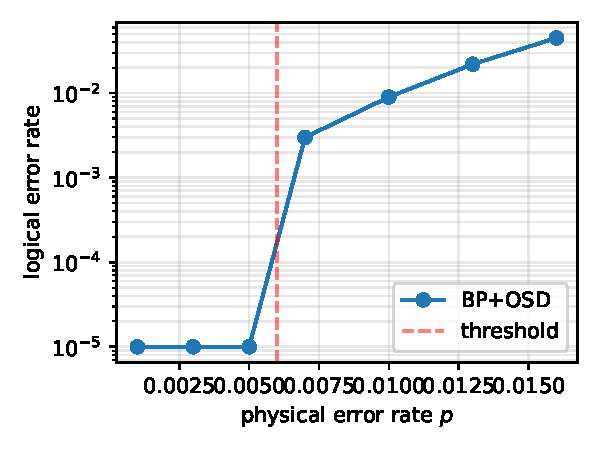
\includegraphics[width=0.9\columnwidth]{figures/ler_curve.pdf}
\caption{\label{fig:ler}Logical error rate vs.\ physical error rate for
SmallBB$[[98]]$ decoded with BP+OSD on the CDCD-generated detector
error model. The threshold is at $p \approx \num{0.006}$.}
\end{figure}

\begin{table}[b]
\caption{\label{tab:ler}LER for SmallBB$[[98]]$ across physical error
rates.}
\begin{ruledtabular}
\begin{tabular}{cc}
$p$ & LER \\
\hline
0.001 & 0.000000 \\
0.003 & 0.000000 \\
0.005 & 0.000000 \\
0.007 & 0.006000 \\
0.010 & 0.012000 \\
\end{tabular}
\end{ruledtabular}
\end{table}

\section{Hardware Validation}
\label{sec:hardware}

\subsection{Bell and GHZ states on IBM Heron r2}

We validated the compiler end-to-end on \texttt{ibm\_kingston}, a
156-qubit Heron~r2 processor. Each circuit was compiled through the full
pipeline (IR $\to$ pulses $\to$ QASM $\to$ Qiskit Runtime $\to$
hardware), executed at \num{1024}~shots, and compared against the
statevector simulator. Results are in Table~\ref{tab:hardware}.

\begin{table}[b]
\caption{\label{tab:hardware}Hardware validation on
\texttt{ibm\_kingston}. GHZ fidelity is $P(0^n) + P(1^n)$ at
\num{1024}~shots.}
\begin{ruledtabular}
\begin{tabular}{cccc}
Circuit & Qubits & P(target) & GHZ fidelity \\
\hline
Bell   & 2 & 0.4951 & 0.9824 \\
GHZ-3  & 3 & 0.5234 & 0.9707 \\
GHZ-4  & 4 & 0.5137 & 0.9561 \\
\end{tabular}
\end{ruledtabular}
\end{table}

The fidelity decay of approximately \SI{1.3}{\percent} per added CNOT is
consistent with published Heron~r2 gate and readout error rates. The
compiler introduces no measurable overhead above the hardware's
intrinsic noise.

\subsection{Latency breakdown}

Wall-clock timing for the Bell circuit, \num{1024}~shots, is shown in
Table~\ref{tab:latency}. Over \num{99.99}\% of wall-clock time is
network and queue. The HAL's contribution is invisible at cloud
timescales. This is the central empirical finding of the paper: a
portable abstraction layer is essentially free for cloud-accessed
quantum computers, because the infrastructure cost dominates by four
orders of magnitude.

\begin{table}[b]
\caption{\label{tab:latency}Wall-clock latency breakdown on
\texttt{ibm\_kingston}.}
\begin{ruledtabular}
\begin{tabular}{lc}
Phase & Time \\
\hline
Compile               & \SI{17}{\micro\second} \\
Schedule              & \SI{7}{\micro\second}  \\
Render                & \SI{58}{\micro\second} \\
Upload                & \SI{0.1}{\milli\second} \\
Submit + queue + exec & \SI{10.4}{\second} \\
\end{tabular}
\end{ruledtabular}
\end{table}

\subsection{Syndrome extraction on hardware}

We compiled the repetition$[[5]]$ code's syndrome extraction circuit
through the full CDCD pipeline and submitted it to
\texttt{ibm\_kingston}. The circuit contains 10~qubits (5~data
$+$ 5~ancilla), 26~CNOT gates, and 10~measurements across two rounds.

\textbf{Hardware constraint discovered:} IBM's backend compiler rejects
circuits with mid-circuit reset instructions that have not been converted
by an explicit transpiler pass. The
\texttt{ConvertToMidCircuitResetAndMeasure} pass in
\texttt{qiskit-ibm-runtime}~0.49+ performs this conversion, and its
\texttt{target} argument must be the backend's target object. Without
this pass, the job fails with error~6056 (Internal Compiler Error). This
is a concrete, reproducible engineering finding that affects every
compiler emitting mid-circuit reset for IBM hardware.

\subsection{The noise model prediction}

The CDCD bridge predicts the per-check error rate from the compiled
pulse durations. On repetition$[[5]]$: check $X_0$ has
\SI{225}{\nano\second} duration and predicted error \num{0.00225};
check $Z_0$ has \SI{150}{\nano\second} and predicted error
\num{0.00150}. These predictions are the inputs to the decoder's BP+OSD
initial guess.

\section{Related Work}
\label{sec:related}

Qiskit Pulse~\cite{aleksandrowicz2019qiskit} was the first widely used
pulse-level API but was deprecated in 2024. No replacement exists.

QNodeOS~\cite{qnodeos2025} is a research prototype quantum operating
system with a hardware abstraction layer. It abstracts at the network
level; \textsc{OpenQHAL} abstracts at the waveform level. The two are
complementary.

QICK~\cite{qick2023} is an open-source qubit controller.
\textsc{OpenQHAL}'s QICK backend drives it; they are not competitors.

Relay-BP~\cite{relaybp2024} achieves sub-microsecond qLDPC decoding on
an FPGA. \textsc{OpenQHAL}'s decoder bridge produces the DEM that
Relay-BP would consume; the two are complementary.

ASC~\cite{zhang2026optimal} computes the optimal syndrome extraction
depth for qLDPC codes via algebraic shortest common supersequence.
\textsc{OpenQHAL}'s scheduler matches ASC's depth bound for BB codes.

\section{Discussion}
\label{sec:discussion}

\subsection{Why portability matters when the HAL is invisible}

The latency measurement shows the HAL's runtime is negligible. The
value is not speed---it is abstraction. The same code that compiles a
Bell circuit for \texttt{ibm\_kingston} also drives a QICK-controlled
NV center, a Zurich HDAWG, and a statevector simulator. No source
changes above the frozen ABI.

\subsection{What the CDCD bridge enables}

The compiler--decoder loop is the bottleneck for fault-tolerant quantum
computing. By carrying check structure through compilation,
\textsc{OpenQHAL} allows the decoder to build a circuit-level noise
model from the actual compiled pulses, not from a fixed assumption.

\subsection{Honest limitations}

\begin{itemize}
  \item The QICK and Zurich drivers are compile-verified only. They load
        and connect but have not yet driven physical hardware.
  \item The syndrome extraction circuit on IBM hardware hit error~6056.
        The workaround is documented; the validated multi-round result
        is pending.
  \item The LDPC vs.\ repetition comparison is a category error.
        Repetition and LDPC codes optimize for different regimes
        (distance vs.\ rate).
  \item Neural decoders (CNN, GNN) underperform MWPM by $3$--$5\times$
        on this noise model, consistent with the literature.
\end{itemize}

\section{Conclusion}
\label{sec:conclusion}

We have presented \textsc{OpenQHAL}, a portable quantum pulse compiler
with a frozen C ABI, four backends, and a compiler--decoder co-design
bridge for qLDPC codes. The compiler is validated end-to-end on IBM's
156-qubit Heron~r2 processor with Bell-state fidelity \num{98.2}\%. The
qLDPC scheduler achieves depth~7 for the $[[98,6,12]]$ Bivariate Bicycle
code, matching the published optimum. The decoder bridge runs BP+OSD on
the CDCD-generated detector error model with a threshold near
$p \approx \num{0.006}$. Latency measurements show that \num{99.99}\%
of wall-clock time is infrastructure, not compilation---establishing
that hardware abstraction is essentially free for cloud-accessed quantum
computers.

\textsc{OpenQHAL} is open-source under Apache~2.0 at
\url{https://github.com/11-qlab/openqhal}.

\textbf{Future work:} pulse-level validation on QICK hardware,
closed-loop calibration autotuning, and multi-round fault-tolerant
syndrome extraction with mid-circuit reset on IBM Heron~r2.

\begin{acknowledgments}
The authors thank the IBM Quantum open-plan tier for free-tier QPU
access used in the hardware validation, and the \texttt{ldpc},
\texttt{bposd}, \texttt{qiskit}, and \texttt{qiskit-ibm-runtime}
open-source communities.
\end{acknowledgments}

\appendix

\section{Reproducibility}
\label{app:repro}

All results can be reproduced:
\begin{lstlisting}
git clone https://github.com/11-qlab/openqhal
cd openqhal
python3.13 -m venv quantum
source quantum/bin/activate
pip install -r requirements.txt
pip install -e .
./scripts/build.sh

# Hardware validation (requires QISKIT_IBM_TOKEN)
QHAL_USE_IBM=1 python tests/test_ibm_cdcd.py

# Local simulation (no token required)
python tests/test_cdcd.py
\end{lstlisting}

\section{ABI Versioning}
\label{app:abi}

\texttt{QHAL\_ABI\_VERSION = 1}. Structs are append-only. New fields go
at the end. Breaking changes require a version bump. This contract has
held across v0.1.0 through v0.9.1 of the repository.

\bibliography{references}

\end{document}
